\documentclass[english]{article}
 
\usepackage{minted}
\usepackage{graphicx}


\begin{document}

\title{ Bench-marking processing performance}

\maketitle  


\section{Bench-marking and environment details:}
%\subsection{}
\begin{itemize}
    \item where do we run the job
    \item how much memory and how much processing the RASCIL imaging script is using
    \item highly parallel so we may be able to use many processor nodes - how much memory do we
need?
    \item profiling doing: benchmarks in the memory and efficiency use of nodes
\end{itemize}

\subsection{Rules IRIS imaging script}
\begin{itemize}
    \item we have the component to run it: eg. RASCIL container on CVMFS
    \item the user provides script and data
    \item we provide: 
    \begin{itemize}
        \item the .jdl model
        \item the singularity container on CVMFS (always latest release) :
        \item environment has to be fully specified in container
        \item the container doesn't need to be uploaded by the user 
    \end{itemize}
\end{itemize}

\subsection{The .jdl model rules:}
\begin{itemize}
    \item the singularity container has to be on CVMFS (always latest release)
    \item scripts should be only input sandbox (not on InputData)
    \item large input/output datasets and data (including .tar .gz) should be on file catalogue only (LFN) - use InputData and OutputData parameters
    \item OutputSandbox can contain standard output (StdOut), standard error (StdErr), small log files, job.info etc (only small files outputs)
\end{itemize}


\section{The .jdl and .sh models samples} 

\hspace{3cm}

\textbf{Specific .jdl model with test data set for efficiency use of nodes:} 
\newline
\begin{minted}{python}
jobName = "%n_RASCILpipeline";

Parameters=3;
ParameterStart=1;
ParameterStep=1;

Executable = "trial.sh";

StdOutput = "StdOut_%n";
StdError = "StdErr_%n";

Tags = {"8Processors","skatelescope.eu.hmem"}; # 2Processors, 4Processors,..,32Processors

SitesList = "LCG.UKI-NORTHGRID-MAN-HEP.uk";
SEList = "UKI-NORTHGRID-MAN-HEP-disk";

InputSandbox = {"trial.sh","input_file1.json"};
InputData = {"LFN:/skatelescope.eu/user/c/cimpan/rascil/
emerlin_rascil_pipeline_for1252_1.tar",
"LFN:/skatelescope.eu/user/w/willice.obonyo/IRIS_RASCIL_test/1252+5634.tar"};

OutputSandbox = {"StdOut_%n","StdErr_%n","*.log"};
OutputData = {"outputs.tar"};

OutputSE = "UKI-NORTHGRID-MAN-HEP-disk";

\end{minted}

\hspace{4cm}

\textbf{Specific .jdl model with test data set for memory benchmark:} 
\newline
\begin{minted}{python}
jobName = "RASCILpipeline";

Executable = "trial.sh";

StdOutput = "StdOut";
StdError = "StdErr";

Tags = {"8Processors","skatelescope.eu.hmem"};

SitesList = "LCG.UKI-NORTHGRID-MAN-HEP.uk";
SEList = "UKI-NORTHGRID-MAN-HEP-disk";

InputSandbox = {"trial.sh","input_file1.json"};
InputData = {"LFN:/skatelescope.eu/user/c/cimpan/rascil/
prmon_2.0.2_x86_64-static-gnu93-opt.tar.gz",
"LFN:/skatelescope.eu/user/c/cimpan/rascil/emerlin_rascil_pipeline_for1252_1.tar",
"LFN:/skatelescope.eu/user/w/willice.obonyo/IRIS_RASCIL_test/1252+5634.tar"};

OutputSandbox = {"StdOut","StdErr","job.info","*.log"};
OutputData = {"outputs.tar","prmon.txt","prmon.json"};

OutputSE = "UKI-NORTHGRID-MAN-HEP-disk";
\end{minted}

\hspace{4cm}

\textbf{Specific .sh model used for both .jdl above:} 
\begin{minted}{python}
vi trial.sh
#printenv;
echo "==============================================";
singularity --version;

echo "Printing parameters"
echo $0
echo $1 #nprocs
echo $2 #id_start
echo $3 #id_end
echo $4 #experiment
echo "Processors: ${OMP_NUM_THREADS}";

tar -xzvf 1252+5634.tar
tar -xzvf emerlin_rascil_pipeline_for1252_1.tar

echo "Extracting Process Monitor - This is to monitor the processes that we will run"

mkdir -p prmon && tar xf prmon_2.0.2_x86_64-static-gnu93-opt.tar.gz -C prmon
--strip-components 1

echo "Running prmon"
./prmon/bin/prmon -p $$ -i 0 -u &


time singularity exec --cleanenv -H $PWD:/srv --pwd /srv -C
/cvmfs/sw.skatelescope.eu/images/rascil.img python3
emerlin_rascil_pipeline/erp2_script.py --params input_file1.json

tar czf outputs.tar *.fits
\end{minted}

\subsection{How .jdl model for efficiency use of nodes (modelcpu.jdl) works:}

The .jdl can be used for 2Processors, 4Processors,..,32Processors
Parameters=3; means 3 jobs will be submitted (you can also choose Parameters=10);
\newline
\begin{minted}{python}
bash-4.2$ dirac-wms-job-submit modelcpu.jdl
JobID = [26381707, 26381708, 26381709]
Output data and logs
bash-4.2$ dirac-wms-job-get-output 26381829
bash-4.2$ dirac-wms-job-get-output-data 26381829
Job 26381829 output data retrieved
bash-4.2$ ls
erp.log outputs.tar StdErr_2 StdOut_2
bash-4.2$ tar -xzvf outputs.tar
eMERLIN_testing_pipeline_1252+5634_cip_deconvolved_moment0.fits
eMERLIN_testing_pipeline_1252+5634_cip_residual_moment0.fits
eMERLIN_testing_pipeline_1252+5634_cip_restored_moment0.fits
\end{minted}


\begin{minted}{python}
We use the benchmarking script:
bash-4.2$ ./benchm 26381707 26381708 26381709
\end{minted}

The output is stored in paramslog.csv (see Figure \ref{fig:param}), which can be opened on own workstation using Excel.
  \begin{figure}[h]
    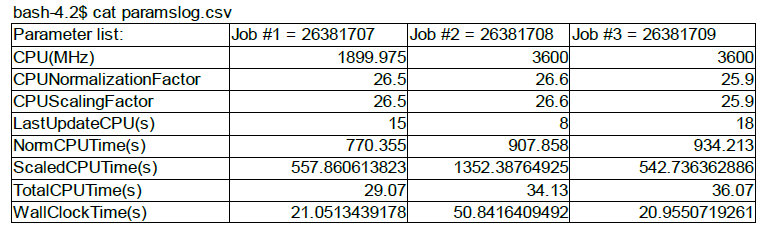
\includegraphics[scale=0.5]{table.png}
\caption{Jobs parameters}
\label{fig:param}
\end{figure}


Efficiency is calculated as TotalCPUTime(s)/(WallClockTime(s)*Number of Processors)
Mean and standard deviation can be calculated on efficiency and then error bars can be plotted
against mean WallClockTime(s). Below is a plot for 10 jobs ran on processors 2 to 32 (see Figure \ref{fig:meaneff}).

\begin{figure}[h]
    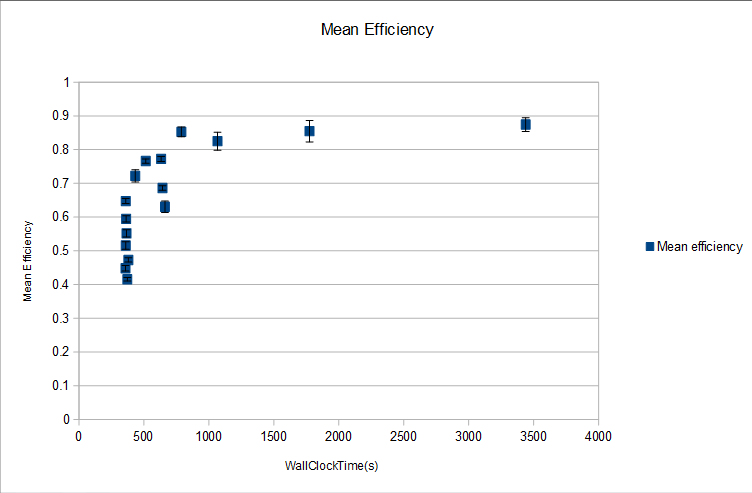
\includegraphics[scale=0.5]{1252meaneff.png}
\caption{TotalCPUTime(s)/(WallClockTime(s)*Number of Processors)}
\label{fig:meaneff}
\end{figure}


\subsection{How .jdl model for efficiency use of nodes (modelm.jdl) works:}
The model outputs files like "prmon.txt","prmon.json" where "prmon.txt" can be plotted using “prmon\_plot.py”
Example of plots are in Figure \ref{fig:pr1252}:
\begin{figure}[h]
    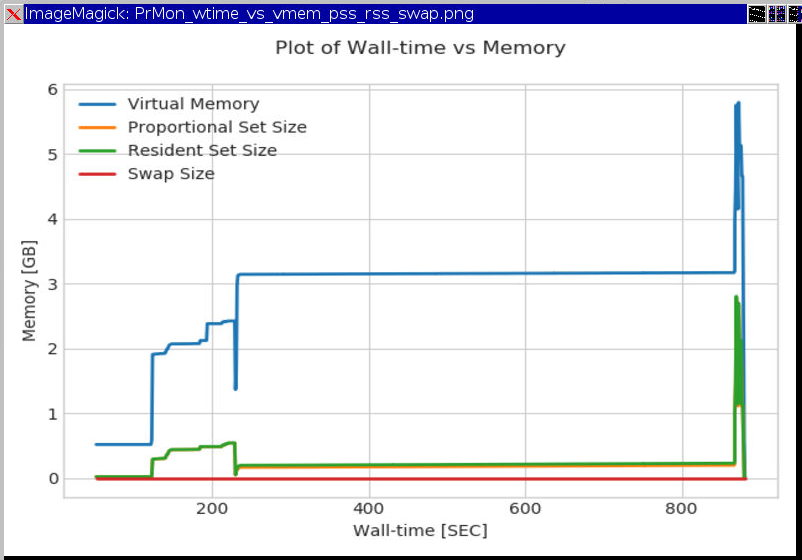
\includegraphics[scale=0.5]{pr1252.png}
\caption{TotalCPUTime(s)/(WallClockTime(s)*Number of Processors)}
\label{fig:pr1252}
\end{figure}


\end{document}
